\documentclass[twoside]{book}

% Packages required by doxygen
\usepackage{calc}
\usepackage{doxygen}
\usepackage{graphicx}
\usepackage[utf8]{inputenc}
\usepackage{makeidx}
\usepackage{multicol}
\usepackage{multirow}
\usepackage{textcomp}
\usepackage[table]{xcolor}

% Font selection
\usepackage[T1]{fontenc}
\usepackage{mathptmx}
\usepackage[scaled=.90]{helvet}
\usepackage{courier}
\usepackage{amssymb}
\usepackage{sectsty}
\renewcommand{\familydefault}{\sfdefault}
\allsectionsfont{%
  \fontseries{bc}\selectfont%
  \color{darkgray}%
}
\renewcommand{\DoxyLabelFont}{%
  \fontseries{bc}\selectfont%
  \color{darkgray}%
}

% Page & text layout
\usepackage{geometry}
\geometry{%
  a4paper,%
  top=2.5cm,%
  bottom=2.5cm,%
  left=2.5cm,%
  right=2.5cm%
}
\tolerance=750
\hfuzz=15pt
\hbadness=750
\setlength{\emergencystretch}{15pt}
\setlength{\parindent}{0cm}
\setlength{\parskip}{0.2cm}
\makeatletter
\renewcommand{\paragraph}{%
  \@startsection{paragraph}{4}{0ex}{-1.0ex}{1.0ex}{%
    \normalfont\normalsize\bfseries\SS@parafont%
  }%
}
\renewcommand{\subparagraph}{%
  \@startsection{subparagraph}{5}{0ex}{-1.0ex}{1.0ex}{%
    \normalfont\normalsize\bfseries\SS@subparafont%
  }%
}
\makeatother

% Headers & footers
\usepackage{fancyhdr}
\pagestyle{fancyplain}
\fancyhead[LE]{\fancyplain{}{\bfseries\thepage}}
\fancyhead[CE]{\fancyplain{}{}}
\fancyhead[RE]{\fancyplain{}{\bfseries\leftmark}}
\fancyhead[LO]{\fancyplain{}{\bfseries\rightmark}}
\fancyhead[CO]{\fancyplain{}{}}
\fancyhead[RO]{\fancyplain{}{\bfseries\thepage}}
\fancyfoot[LE]{\fancyplain{}{}}
\fancyfoot[CE]{\fancyplain{}{}}
\fancyfoot[RE]{\fancyplain{}{\bfseries\scriptsize Generated on Tue Dec 12 2017 14\-:00\-:00 for My Project by Doxygen }}
\fancyfoot[LO]{\fancyplain{}{\bfseries\scriptsize Generated on Tue Dec 12 2017 14\-:00\-:00 for My Project by Doxygen }}
\fancyfoot[CO]{\fancyplain{}{}}
\fancyfoot[RO]{\fancyplain{}{}}
\renewcommand{\footrulewidth}{0.4pt}
\renewcommand{\chaptermark}[1]{%
  \markboth{#1}{}%
}
\renewcommand{\sectionmark}[1]{%
  \markright{\thesection\ #1}%
}

% Indices & bibliography
\usepackage{natbib}
\usepackage[titles]{tocloft}
\setcounter{tocdepth}{3}
\setcounter{secnumdepth}{5}
\makeindex

% Hyperlinks (required, but should be loaded last)
\usepackage{ifpdf}
\ifpdf
  \usepackage[pdftex,pagebackref=true]{hyperref}
\else
  \usepackage[ps2pdf,pagebackref=true]{hyperref}
\fi
\hypersetup{%
  colorlinks=true,%
  linkcolor=blue,%
  citecolor=blue,%
  unicode%
}

% Custom commands
\newcommand{\clearemptydoublepage}{%
  \newpage{\pagestyle{empty}\cleardoublepage}%
}


%===== C O N T E N T S =====

\begin{document}

% Titlepage & ToC
\hypersetup{pageanchor=false}
\pagenumbering{roman}
\begin{titlepage}
\vspace*{7cm}
\begin{center}%
{\Large My Project }\\
\vspace*{1cm}
{\large Generated by Doxygen 1.8.6}\\
\vspace*{0.5cm}
{\small Tue Dec 12 2017 14:00:00}\\
\end{center}
\end{titlepage}
\clearemptydoublepage
\tableofcontents
\clearemptydoublepage
\pagenumbering{arabic}
\hypersetup{pageanchor=true}

%--- Begin generated contents ---
\chapter{Hierarchical Index}
\section{Class Hierarchy}
This inheritance list is sorted roughly, but not completely, alphabetically\-:\begin{DoxyCompactList}
\item \contentsline{section}{Administateur}{\pageref{classAdministateur}}{}
\item \contentsline{section}{Cours}{\pageref{classCours}}{}
\item \contentsline{section}{Utilisateur}{\pageref{classUtilisateur}}{}
\begin{DoxyCompactList}
\item \contentsline{section}{Administrateur}{\pageref{classAdministrateur}}{}
\item \contentsline{section}{Enseignant}{\pageref{classEnseignant}}{}
\item \contentsline{section}{Etudiant}{\pageref{classEtudiant}}{}
\end{DoxyCompactList}
\item \contentsline{section}{Utilisateur\-Abstract\-Factory}{\pageref{classUtilisateurAbstractFactory}}{}
\begin{DoxyCompactList}
\item \contentsline{section}{Administrateur\-Concrete\-Factory}{\pageref{classAdministrateurConcreteFactory}}{}
\item \contentsline{section}{Enseignant\-Concrete\-Factory}{\pageref{classEnseignantConcreteFactory}}{}
\item \contentsline{section}{Etudiant\-Concrete\-Factory}{\pageref{classEtudiantConcreteFactory}}{}
\end{DoxyCompactList}
\end{DoxyCompactList}

\chapter{Class Index}
\section{Class List}
Here are the classes, structs, unions and interfaces with brief descriptions\-:\begin{DoxyCompactList}
\item\contentsline{section}{\hyperlink{classAdministateur}{Administateur} \\*Classe concrete \hyperlink{classAdministateur}{Administateur} }{\pageref{classAdministateur}}{}
\item\contentsline{section}{\hyperlink{classAdministrateur}{Administrateur} }{\pageref{classAdministrateur}}{}
\item\contentsline{section}{\hyperlink{classAdministrateurConcreteFactory}{Administrateur\-Concrete\-Factory} }{\pageref{classAdministrateurConcreteFactory}}{}
\item\contentsline{section}{\hyperlink{classCours}{Cours} \\*Classe cours }{\pageref{classCours}}{}
\item\contentsline{section}{\hyperlink{classEnseignant}{Enseignant} \\*Classe enseignant }{\pageref{classEnseignant}}{}
\item\contentsline{section}{\hyperlink{classEnseignantConcreteFactory}{Enseignant\-Concrete\-Factory} }{\pageref{classEnseignantConcreteFactory}}{}
\item\contentsline{section}{\hyperlink{classEtudiant}{Etudiant} \\*Classe \hyperlink{classEtudiant}{Etudiant} }{\pageref{classEtudiant}}{}
\item\contentsline{section}{\hyperlink{classEtudiantConcreteFactory}{Etudiant\-Concrete\-Factory} }{\pageref{classEtudiantConcreteFactory}}{}
\item\contentsline{section}{\hyperlink{classUtilisateur}{Utilisateur} \\*Classe utilisateur }{\pageref{classUtilisateur}}{}
\item\contentsline{section}{\hyperlink{classUtilisateurAbstractFactory}{Utilisateur\-Abstract\-Factory} }{\pageref{classUtilisateurAbstractFactory}}{}
\end{DoxyCompactList}

\chapter{File Index}
\section{File List}
Here is a list of all documented files with brief descriptions\-:\begin{DoxyCompactList}
\item\contentsline{section}{{\bfseries Administrateur.\-hpp} }{\pageref{Administrateur_8hpp}}{}
\item\contentsline{section}{\hyperlink{Cours_8hpp}{Cours.\-hpp} \\*Classe cours }{\pageref{Cours_8hpp}}{}
\item\contentsline{section}{\hyperlink{Enseignant_8hpp}{Enseignant.\-hpp} \\*Classe enseignant }{\pageref{Enseignant_8hpp}}{}
\item\contentsline{section}{\hyperlink{Etudiant_8hpp}{Etudiant.\-hpp} \\*Classe \hyperlink{classEtudiant}{Etudiant} }{\pageref{Etudiant_8hpp}}{}
\item\contentsline{section}{\hyperlink{Utilisateur_8hpp}{Utilisateur.\-hpp} \\*Classe abstraite utilisateur }{\pageref{Utilisateur_8hpp}}{}
\item\contentsline{section}{\hyperlink{UtilisateurAbstractFactory_8hpp}{Utilisateur\-Abstract\-Factory.\-hpp} }{\pageref{UtilisateurAbstractFactory_8hpp}}{}
\end{DoxyCompactList}

\chapter{Class Documentation}
\hypertarget{classAdministateur}{\section{Administateur Class Reference}
\label{classAdministateur}\index{Administateur@{Administateur}}
}


Classe concrete \hyperlink{classAdministateur}{Administateur}.  




{\ttfamily \#include $<$Administrateur.\-hpp$>$}



\subsection{Detailed Description}
Classe concrete \hyperlink{classAdministateur}{Administateur}. 

Permet d'instancier un utilisateur \hyperlink{classAdministateur}{Administateur} avec un num\-Admin spécifique 

The documentation for this class was generated from the following file\-:\begin{DoxyCompactItemize}
\item 
Administrateur.\-hpp\end{DoxyCompactItemize}

\hypertarget{classAdministrateur}{\section{Administrateur Class Reference}
\label{classAdministrateur}\index{Administrateur@{Administrateur}}
}
Inheritance diagram for Administrateur\-:\begin{figure}[H]
\begin{center}
\leavevmode
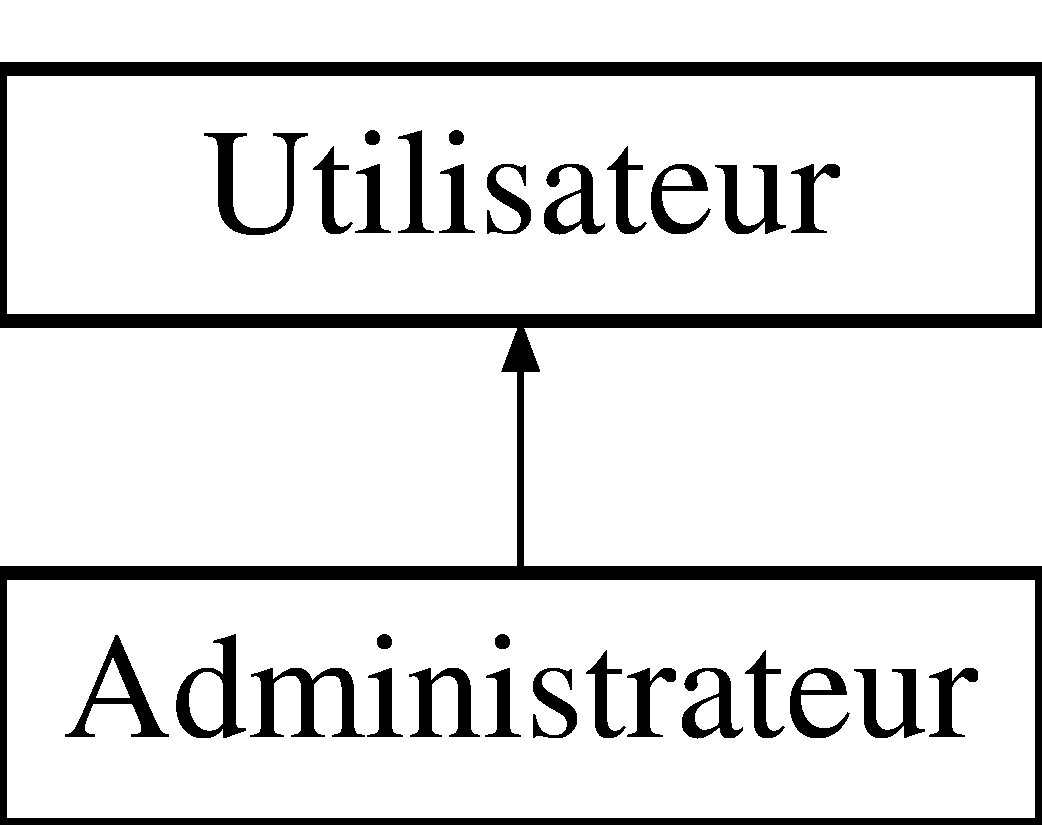
\includegraphics[height=2.000000cm]{classAdministrateur}
\end{center}
\end{figure}
\subsection*{Public Member Functions}
\begin{DoxyCompactItemize}
\item 
\hyperlink{classAdministrateur_a08dc2614d133d65ffa1913ed85f200fd}{Administrateur} (std\-::string n, std\-::string p, struct tm d)
\begin{DoxyCompactList}\small\item\em Constructeur de la classe \hyperlink{classAdministateur}{Administateur}. \end{DoxyCompactList}\item 
\hyperlink{classAdministrateur_af11ee7b63aabe45c5c2aa0532db1c7db}{$\sim$\-Administrateur} ()
\begin{DoxyCompactList}\small\item\em Destructeur. \end{DoxyCompactList}\item 
\hypertarget{classAdministrateur_a5183b877b2a8aa3d5951e06f453dd622}{void \hyperlink{classAdministrateur_a5183b877b2a8aa3d5951e06f453dd622}{print} ()}\label{classAdministrateur_a5183b877b2a8aa3d5951e06f453dd622}

\begin{DoxyCompactList}\small\item\em Affiche des informations sur l'\hyperlink{classAdministrateur}{Administrateur}. \end{DoxyCompactList}\end{DoxyCompactItemize}
\subsection*{Additional Inherited Members}


\subsection{Constructor \& Destructor Documentation}
\hypertarget{classAdministrateur_a08dc2614d133d65ffa1913ed85f200fd}{\index{Administrateur@{Administrateur}!Administrateur@{Administrateur}}
\index{Administrateur@{Administrateur}!Administrateur@{Administrateur}}
\subsubsection[{Administrateur}]{\setlength{\rightskip}{0pt plus 5cm}Administrateur\-::\-Administrateur (
\begin{DoxyParamCaption}
\item[{std\-::string}]{n, }
\item[{std\-::string}]{p, }
\item[{struct tm}]{d}
\end{DoxyParamCaption}
)\hspace{0.3cm}{\ttfamily [inline]}}}\label{classAdministrateur_a08dc2614d133d65ffa1913ed85f200fd}


Constructeur de la classe \hyperlink{classAdministateur}{Administateur}. 


\begin{DoxyParams}{Parameters}
{\em n} & Nom de l'\hyperlink{classAdministateur}{Administateur} \\
\hline
{\em p} & Prénom de l'administrateur \\
\hline
{\em d} & Date de naissance de l'administrateur \\
\hline
\end{DoxyParams}
\hypertarget{classAdministrateur_af11ee7b63aabe45c5c2aa0532db1c7db}{\index{Administrateur@{Administrateur}!$\sim$\-Administrateur@{$\sim$\-Administrateur}}
\index{$\sim$\-Administrateur@{$\sim$\-Administrateur}!Administrateur@{Administrateur}}
\subsubsection[{$\sim$\-Administrateur}]{\setlength{\rightskip}{0pt plus 5cm}Administrateur\-::$\sim$\-Administrateur (
\begin{DoxyParamCaption}
{}
\end{DoxyParamCaption}
)}}\label{classAdministrateur_af11ee7b63aabe45c5c2aa0532db1c7db}


Destructeur. 

Destructeur de l'administrateur (appelè avant celui d'\hyperlink{classUtilisateur}{Utilisateur}) 

The documentation for this class was generated from the following file\-:\begin{DoxyCompactItemize}
\item 
Administrateur.\-hpp\end{DoxyCompactItemize}

\hypertarget{classAdministrateurConcreteFactory}{\section{Administrateur\-Concrete\-Factory Class Reference}
\label{classAdministrateurConcreteFactory}\index{Administrateur\-Concrete\-Factory@{Administrateur\-Concrete\-Factory}}
}
Inheritance diagram for Administrateur\-Concrete\-Factory\-:\begin{figure}[H]
\begin{center}
\leavevmode
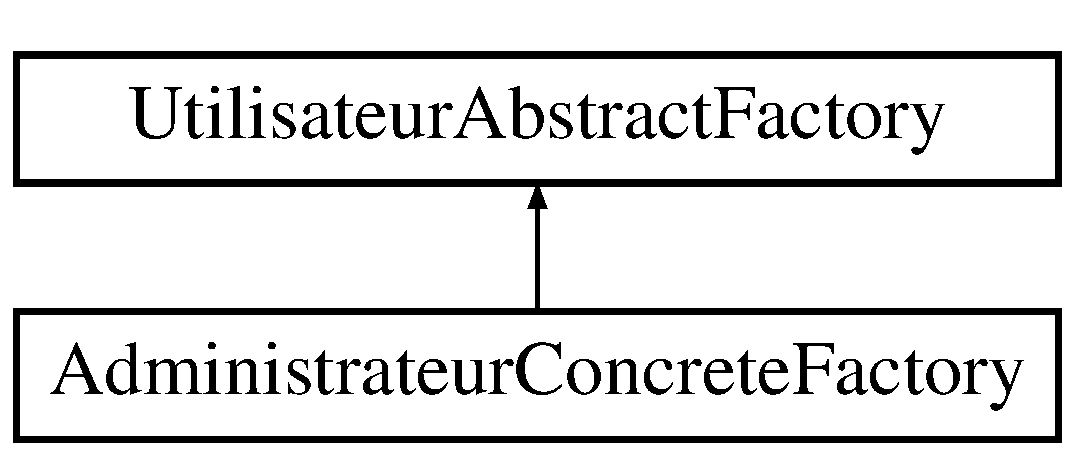
\includegraphics[height=2.000000cm]{classAdministrateurConcreteFactory}
\end{center}
\end{figure}
\subsection*{Public Member Functions}
\begin{DoxyCompactItemize}
\item 
\hypertarget{classAdministrateurConcreteFactory_a17bfd0bf30fbb82ee3053e027a6ca4a8}{\hyperlink{classUtilisateur}{Utilisateur} $\ast$ {\bfseries creer\-Utilisateur} (std\-::string nom, std\-::string prenom)}\label{classAdministrateurConcreteFactory_a17bfd0bf30fbb82ee3053e027a6ca4a8}

\end{DoxyCompactItemize}


The documentation for this class was generated from the following file\-:\begin{DoxyCompactItemize}
\item 
\hyperlink{UtilisateurAbstractFactory_8hpp}{Utilisateur\-Abstract\-Factory.\-hpp}\end{DoxyCompactItemize}

\hypertarget{classCours}{\section{Cours Class Reference}
\label{classCours}\index{Cours@{Cours}}
}


Classe cours.  




{\ttfamily \#include $<$Cours.\-hpp$>$}

\subsection*{Public Member Functions}
\begin{DoxyCompactItemize}
\item 
\hyperlink{classCours_a54d01f69f01be5224bd4a76dd90dedd9}{Cours} (std\-::string nom\-Cours, std\-::string description, struct tm date\-D, struct tm date\-F, struct tm date\-Fin\-Insc, int capa, \hyperlink{classEnseignant}{Enseignant} $\ast$ens)
\begin{DoxyCompactList}\small\item\em Constructeur. \end{DoxyCompactList}\item 
\hyperlink{classCours_a598a1fa3dfe1a337fb07731a51d7da16}{$\sim$\-Cours} ()
\begin{DoxyCompactList}\small\item\em Destructeur. \end{DoxyCompactList}\item 
\hypertarget{classCours_ac0f58aede568d4a8f47f9c4a702fa297}{void \hyperlink{classCours_ac0f58aede568d4a8f47f9c4a702fa297}{print} ()}\label{classCours_ac0f58aede568d4a8f47f9c4a702fa297}

\begin{DoxyCompactList}\small\item\em Affiche des informations sur le cours. \end{DoxyCompactList}\end{DoxyCompactItemize}


\subsection{Detailed Description}
Classe cours. 

Permet de creer un cours en attente de validation, et par la suite de l'ajouter a l'application 

\subsection{Constructor \& Destructor Documentation}
\hypertarget{classCours_a54d01f69f01be5224bd4a76dd90dedd9}{\index{Cours@{Cours}!Cours@{Cours}}
\index{Cours@{Cours}!Cours@{Cours}}
\subsubsection[{Cours}]{\setlength{\rightskip}{0pt plus 5cm}Cours\-::\-Cours (
\begin{DoxyParamCaption}
\item[{std\-::string}]{nom\-Cours, }
\item[{std\-::string}]{description, }
\item[{struct tm}]{date\-D, }
\item[{struct tm}]{date\-F, }
\item[{struct tm}]{date\-Fin\-Insc, }
\item[{int}]{capa, }
\item[{{\bf Enseignant} $\ast$}]{ens}
\end{DoxyParamCaption}
)\hspace{0.3cm}{\ttfamily [inline]}}}\label{classCours_a54d01f69f01be5224bd4a76dd90dedd9}


Constructeur. 

Constructeur de la classe C\-Ours


\begin{DoxyParams}{Parameters}
{\em nom\-Cours} & Nom du cours proposé \\
\hline
{\em description} & Description du \hyperlink{classCours}{Cours} \\
\hline
{\em date\-D} & date de début du \hyperlink{classCours}{Cours} \\
\hline
{\em date\-F} & date de fin du cours \\
\hline
{\em date\-Fin\-Insc} & Date de fin d'inscriptions \\
\hline
{\em capa} & Capacité d'étudiant maximal du cours \\
\hline
\end{DoxyParams}
\hypertarget{classCours_a598a1fa3dfe1a337fb07731a51d7da16}{\index{Cours@{Cours}!$\sim$\-Cours@{$\sim$\-Cours}}
\index{$\sim$\-Cours@{$\sim$\-Cours}!Cours@{Cours}}
\subsubsection[{$\sim$\-Cours}]{\setlength{\rightskip}{0pt plus 5cm}Cours\-::$\sim$\-Cours (
\begin{DoxyParamCaption}
{}
\end{DoxyParamCaption}
)}}\label{classCours_a598a1fa3dfe1a337fb07731a51d7da16}


Destructeur. 

Détruit le cours 

The documentation for this class was generated from the following file\-:\begin{DoxyCompactItemize}
\item 
\hyperlink{Cours_8hpp}{Cours.\-hpp}\end{DoxyCompactItemize}

\hypertarget{classEnseignant}{\section{Enseignant Class Reference}
\label{classEnseignant}\index{Enseignant@{Enseignant}}
}


Classe enseignant.  




{\ttfamily \#include $<$Enseignant.\-hpp$>$}

Inheritance diagram for Enseignant\-:\begin{figure}[H]
\begin{center}
\leavevmode
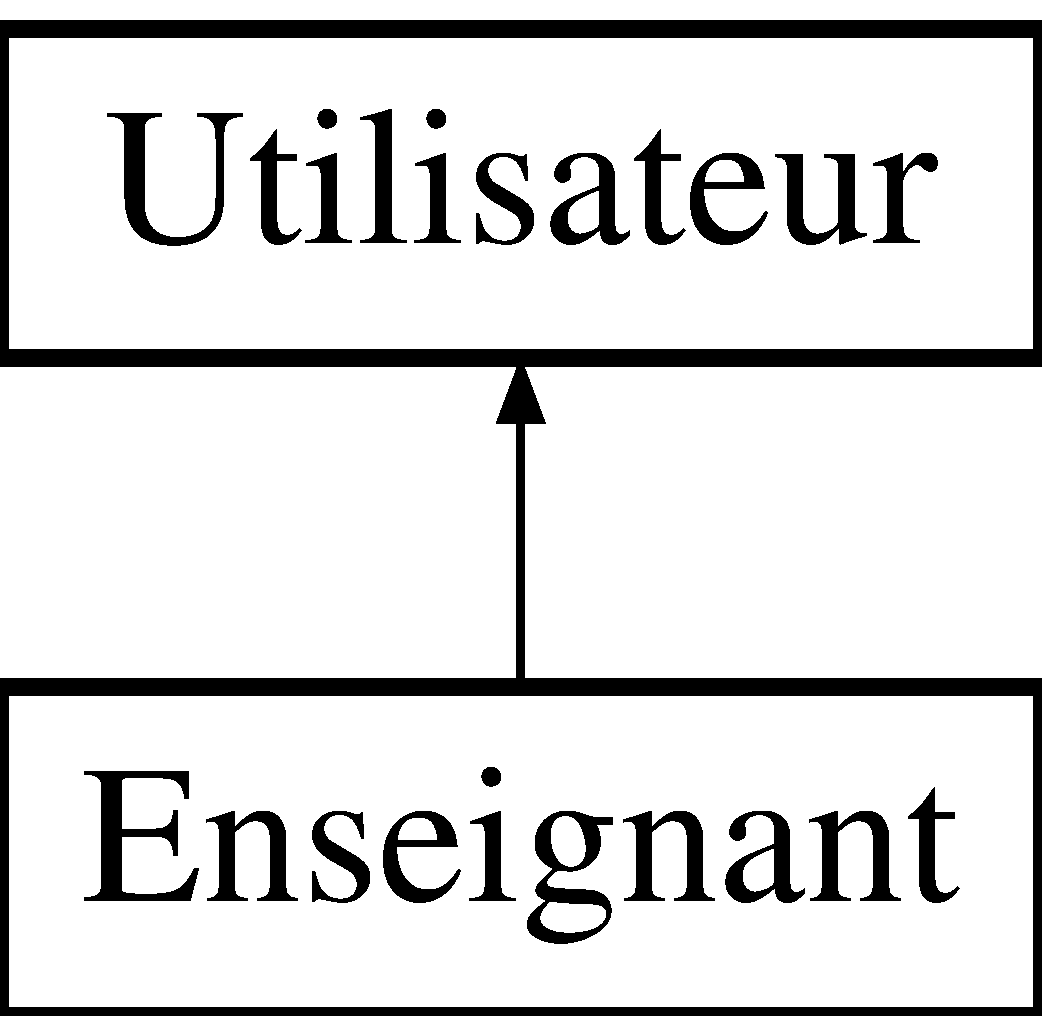
\includegraphics[height=2.000000cm]{classEnseignant}
\end{center}
\end{figure}
\subsection*{Public Member Functions}
\begin{DoxyCompactItemize}
\item 
\hyperlink{classEnseignant_a349f455fe0fbf43a884e2f8a21f057d7}{Enseignant} (std\-::string n, std\-::string pre, struct tm date\-N)
\begin{DoxyCompactList}\small\item\em Constructeur. \end{DoxyCompactList}\item 
\hyperlink{classEnseignant_a9317ba87e8b7e32fa5e48bdbff1c9cce}{$\sim$\-Enseignant} ()
\begin{DoxyCompactList}\small\item\em Destructeur. \end{DoxyCompactList}\item 
\hyperlink{classCours}{Cours} $\ast$ \hyperlink{classEnseignant_a5c39655711ebda90f8568be84fe64872}{proposer\-Cours} (std\-::string nom\-Cours, std\-::string description, struct tm date\-Debut, struct tm date\-Fin, struct tm date\-Fin\-Insc, int nb\-P\-Laces)
\begin{DoxyCompactList}\small\item\em Permet a l'enseignant de creer un cours. \end{DoxyCompactList}\item 
\hypertarget{classEnseignant_af86bb8ab32afabe18507ce5788370c3d}{void \hyperlink{classEnseignant_af86bb8ab32afabe18507ce5788370c3d}{print} ()}\label{classEnseignant_af86bb8ab32afabe18507ce5788370c3d}

\begin{DoxyCompactList}\small\item\em Affiche des informations sur l'\hyperlink{classEnseignant}{Enseignant}. \end{DoxyCompactList}\end{DoxyCompactItemize}
\subsection*{Additional Inherited Members}


\subsection{Detailed Description}
Classe enseignant. 

Permet d'instancier un enseignant avec un num\-Ens spécifique 

\subsection{Constructor \& Destructor Documentation}
\hypertarget{classEnseignant_a349f455fe0fbf43a884e2f8a21f057d7}{\index{Enseignant@{Enseignant}!Enseignant@{Enseignant}}
\index{Enseignant@{Enseignant}!Enseignant@{Enseignant}}
\subsubsection[{Enseignant}]{\setlength{\rightskip}{0pt plus 5cm}Enseignant\-::\-Enseignant (
\begin{DoxyParamCaption}
\item[{std\-::string}]{n, }
\item[{std\-::string}]{pre, }
\item[{struct tm}]{date\-N}
\end{DoxyParamCaption}
)\hspace{0.3cm}{\ttfamily [inline]}}}\label{classEnseignant_a349f455fe0fbf43a884e2f8a21f057d7}


Constructeur. 

Constructeur de la classe \hyperlink{classEnseignant}{Enseignant}


\begin{DoxyParams}{Parameters}
{\em n} & nom de l'enseignant \\
\hline
{\em p} & prenom de l'enseignant \\
\hline
{\em d} & date de naissance de l'enseignant \\
\hline
\end{DoxyParams}
\hypertarget{classEnseignant_a9317ba87e8b7e32fa5e48bdbff1c9cce}{\index{Enseignant@{Enseignant}!$\sim$\-Enseignant@{$\sim$\-Enseignant}}
\index{$\sim$\-Enseignant@{$\sim$\-Enseignant}!Enseignant@{Enseignant}}
\subsubsection[{$\sim$\-Enseignant}]{\setlength{\rightskip}{0pt plus 5cm}Enseignant\-::$\sim$\-Enseignant (
\begin{DoxyParamCaption}
{}
\end{DoxyParamCaption}
)}}\label{classEnseignant_a9317ba87e8b7e32fa5e48bdbff1c9cce}


Destructeur. 

Detruit un enseignant (appelè avant le déstructeur utilisateur) 

\subsection{Member Function Documentation}
\hypertarget{classEnseignant_a5c39655711ebda90f8568be84fe64872}{\index{Enseignant@{Enseignant}!proposer\-Cours@{proposer\-Cours}}
\index{proposer\-Cours@{proposer\-Cours}!Enseignant@{Enseignant}}
\subsubsection[{proposer\-Cours}]{\setlength{\rightskip}{0pt plus 5cm}{\bf Cours}$\ast$ Enseignant\-::proposer\-Cours (
\begin{DoxyParamCaption}
\item[{std\-::string}]{nom\-Cours, }
\item[{std\-::string}]{description, }
\item[{struct tm}]{date\-Debut, }
\item[{struct tm}]{date\-Fin, }
\item[{struct tm}]{date\-Fin\-Insc, }
\item[{int}]{nb\-P\-Laces}
\end{DoxyParamCaption}
)\hspace{0.3cm}{\ttfamily [inline]}}}\label{classEnseignant_a5c39655711ebda90f8568be84fe64872}


Permet a l'enseignant de creer un cours. 


\begin{DoxyParams}{Parameters}
{\em nom\-Cours} & Nom du cours proposé \\
\hline
{\em description} & Description du \hyperlink{classCours}{Cours} \\
\hline
{\em date\-D} & date de début du \hyperlink{classCours}{Cours} \\
\hline
{\em date\-F} & date de fin du cours \\
\hline
{\em date\-Fin\-Insc} & Date de fin d'inscriptions \\
\hline
{\em capa} & Capacité d'étudiant maximal du cours\\
\hline
\end{DoxyParams}
\begin{DoxyReturn}{Returns}
pointeur vers le cours créé 
\end{DoxyReturn}


The documentation for this class was generated from the following file\-:\begin{DoxyCompactItemize}
\item 
\hyperlink{Enseignant_8hpp}{Enseignant.\-hpp}\end{DoxyCompactItemize}

\hypertarget{classEnseignantConcreteFactory}{\section{Enseignant\-Concrete\-Factory Class Reference}
\label{classEnseignantConcreteFactory}\index{Enseignant\-Concrete\-Factory@{Enseignant\-Concrete\-Factory}}
}
Inheritance diagram for Enseignant\-Concrete\-Factory\-:\begin{figure}[H]
\begin{center}
\leavevmode
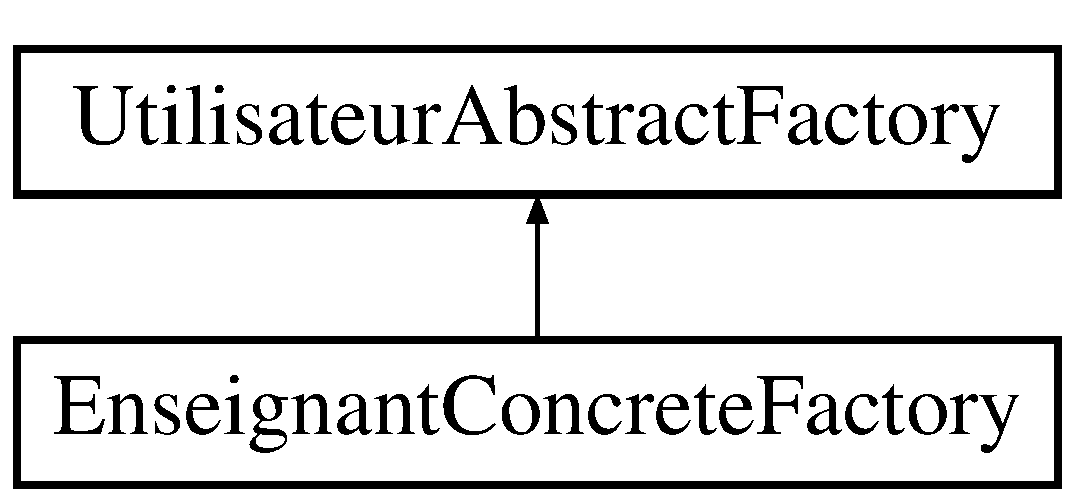
\includegraphics[height=2.000000cm]{classEnseignantConcreteFactory}
\end{center}
\end{figure}
\subsection*{Public Member Functions}
\begin{DoxyCompactItemize}
\item 
\hypertarget{classEnseignantConcreteFactory_a559eaa00e105df593115e0a7c34788cb}{\hyperlink{classUtilisateur}{Utilisateur} $\ast$ {\bfseries creer\-Utilisateur} (std\-::string nom, std\-::string prenom)}\label{classEnseignantConcreteFactory_a559eaa00e105df593115e0a7c34788cb}

\end{DoxyCompactItemize}


The documentation for this class was generated from the following file\-:\begin{DoxyCompactItemize}
\item 
\hyperlink{UtilisateurAbstractFactory_8hpp}{Utilisateur\-Abstract\-Factory.\-hpp}\end{DoxyCompactItemize}

\hypertarget{classEtudiant}{\section{Etudiant Class Reference}
\label{classEtudiant}\index{Etudiant@{Etudiant}}
}


Classe \hyperlink{classEtudiant}{Etudiant}.  




{\ttfamily \#include $<$Etudiant.\-hpp$>$}

Inheritance diagram for Etudiant\-:\begin{figure}[H]
\begin{center}
\leavevmode
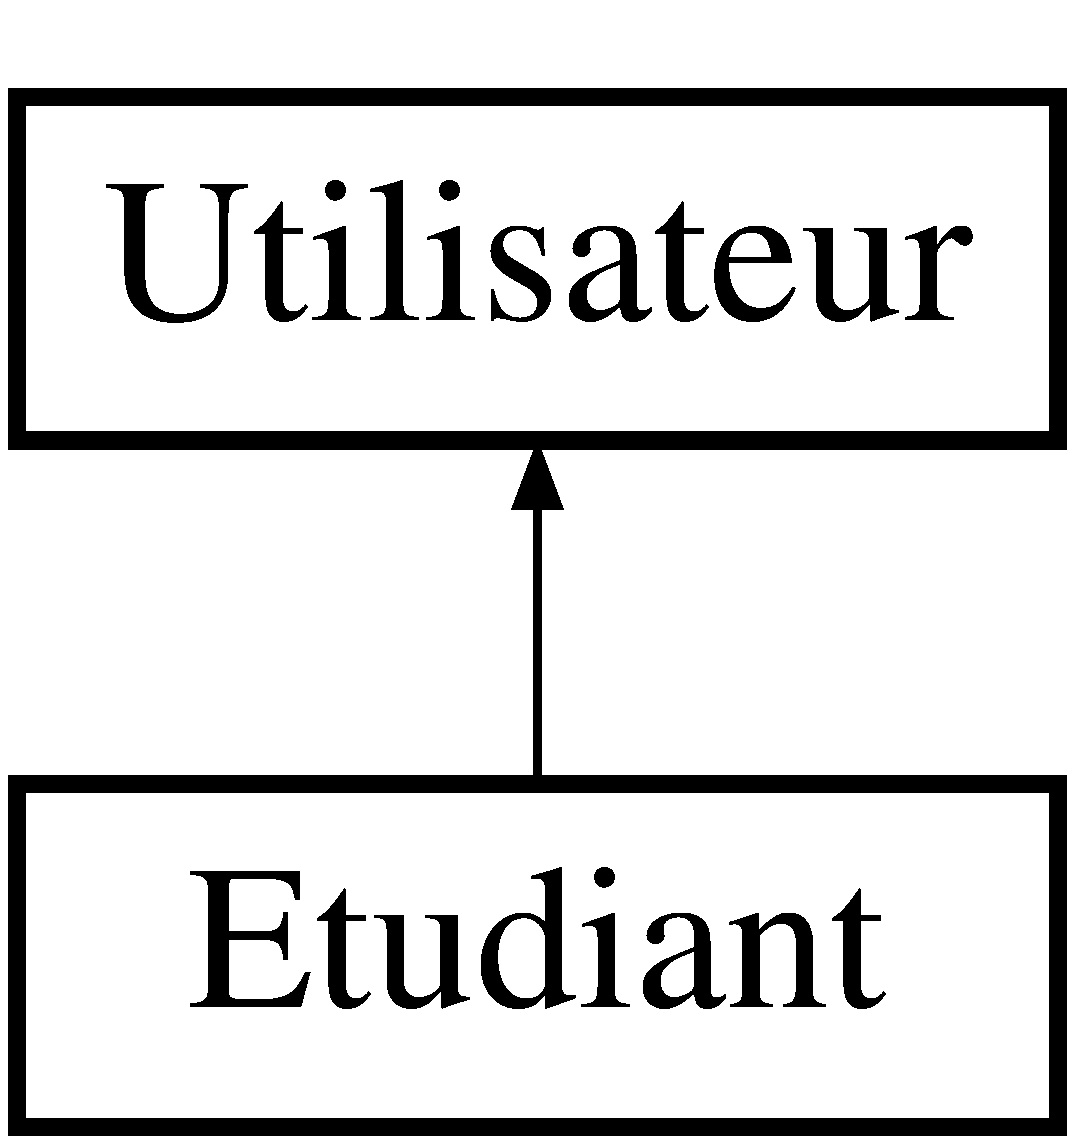
\includegraphics[height=2.000000cm]{classEtudiant}
\end{center}
\end{figure}
\subsection*{Public Member Functions}
\begin{DoxyCompactItemize}
\item 
\hyperlink{classEtudiant_a3074a4459cca24f8862faa7118242e2b}{Etudiant} (std\-::string n, std\-::string p, struct tm d)
\begin{DoxyCompactList}\small\item\em Constructeur. \end{DoxyCompactList}\item 
\hyperlink{classEtudiant_a47bb756690e1389b6fbd1d2f65cd4eac}{$\sim$\-Etudiant} ()
\begin{DoxyCompactList}\small\item\em Destructeur. \end{DoxyCompactList}\item 
\hypertarget{classEtudiant_a4e9a71af9aba98f15b6fbe5bbe41d2d7}{void \hyperlink{classEtudiant_a4e9a71af9aba98f15b6fbe5bbe41d2d7}{print} ()}\label{classEtudiant_a4e9a71af9aba98f15b6fbe5bbe41d2d7}

\begin{DoxyCompactList}\small\item\em Affiche des informations sur l'\hyperlink{classEtudiant}{Etudiant}. \end{DoxyCompactList}\end{DoxyCompactItemize}
\subsection*{Additional Inherited Members}


\subsection{Detailed Description}
Classe \hyperlink{classEtudiant}{Etudiant}. 

Permet d'instancier un étudiant avec un num\-Ine spécifique 

\subsection{Constructor \& Destructor Documentation}
\hypertarget{classEtudiant_a3074a4459cca24f8862faa7118242e2b}{\index{Etudiant@{Etudiant}!Etudiant@{Etudiant}}
\index{Etudiant@{Etudiant}!Etudiant@{Etudiant}}
\subsubsection[{Etudiant}]{\setlength{\rightskip}{0pt plus 5cm}Etudiant\-::\-Etudiant (
\begin{DoxyParamCaption}
\item[{std\-::string}]{n, }
\item[{std\-::string}]{p, }
\item[{struct tm}]{d}
\end{DoxyParamCaption}
)\hspace{0.3cm}{\ttfamily [inline]}}}\label{classEtudiant_a3074a4459cca24f8862faa7118242e2b}


Constructeur. 

Constructeur de la classe \hyperlink{classEtudiant}{Etudiant}


\begin{DoxyParams}{Parameters}
{\em n} & Nom de l'étudiant \\
\hline
{\em p} & Prénom de l'étudiant \\
\hline
{\em d} & Date de naissance de l'étudiant \\
\hline
\end{DoxyParams}
\hypertarget{classEtudiant_a47bb756690e1389b6fbd1d2f65cd4eac}{\index{Etudiant@{Etudiant}!$\sim$\-Etudiant@{$\sim$\-Etudiant}}
\index{$\sim$\-Etudiant@{$\sim$\-Etudiant}!Etudiant@{Etudiant}}
\subsubsection[{$\sim$\-Etudiant}]{\setlength{\rightskip}{0pt plus 5cm}Etudiant\-::$\sim$\-Etudiant (
\begin{DoxyParamCaption}
{}
\end{DoxyParamCaption}
)}}\label{classEtudiant_a47bb756690e1389b6fbd1d2f65cd4eac}


Destructeur. 

Détruit un étudiant (appelé avant le déstructeur d'utilisateur) 

The documentation for this class was generated from the following file\-:\begin{DoxyCompactItemize}
\item 
\hyperlink{Etudiant_8hpp}{Etudiant.\-hpp}\end{DoxyCompactItemize}

\hypertarget{classEtudiantConcreteFactory}{\section{Etudiant\-Concrete\-Factory Class Reference}
\label{classEtudiantConcreteFactory}\index{Etudiant\-Concrete\-Factory@{Etudiant\-Concrete\-Factory}}
}
Inheritance diagram for Etudiant\-Concrete\-Factory\-:\begin{figure}[H]
\begin{center}
\leavevmode
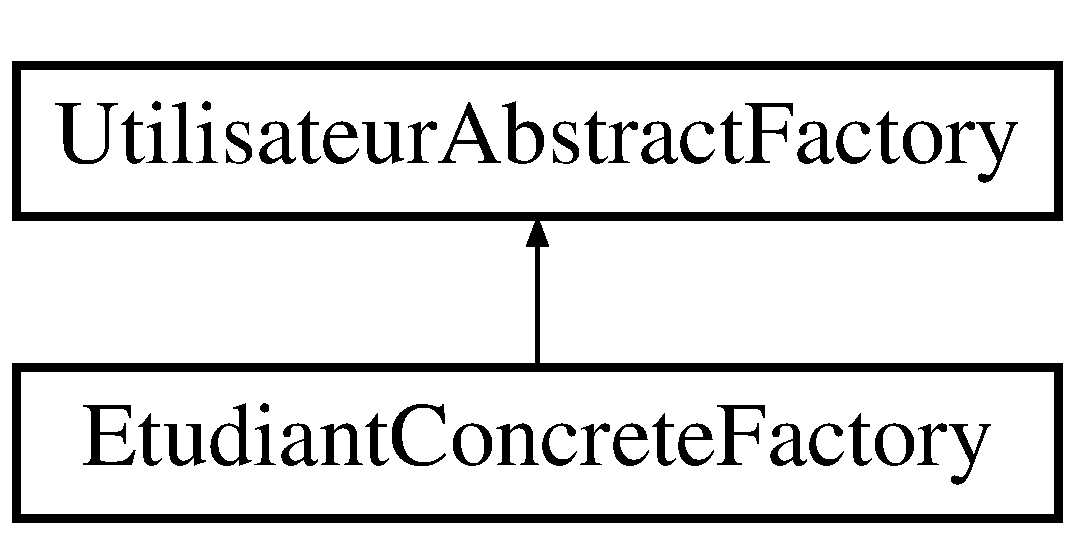
\includegraphics[height=2.000000cm]{classEtudiantConcreteFactory}
\end{center}
\end{figure}
\subsection*{Public Member Functions}
\begin{DoxyCompactItemize}
\item 
\hypertarget{classEtudiantConcreteFactory_a09792abdb4be6bf063d80d5fd9532075}{\hyperlink{classUtilisateur}{Utilisateur} $\ast$ {\bfseries creer\-Utilisateur} (std\-::string nom, std\-::string prenom)}\label{classEtudiantConcreteFactory_a09792abdb4be6bf063d80d5fd9532075}

\end{DoxyCompactItemize}


The documentation for this class was generated from the following file\-:\begin{DoxyCompactItemize}
\item 
\hyperlink{UtilisateurAbstractFactory_8hpp}{Utilisateur\-Abstract\-Factory.\-hpp}\end{DoxyCompactItemize}

\hypertarget{classUtilisateur}{\section{Utilisateur Class Reference}
\label{classUtilisateur}\index{Utilisateur@{Utilisateur}}
}


Classe utilisateur.  




{\ttfamily \#include $<$Utilisateur.\-hpp$>$}

Inheritance diagram for Utilisateur\-:\begin{figure}[H]
\begin{center}
\leavevmode
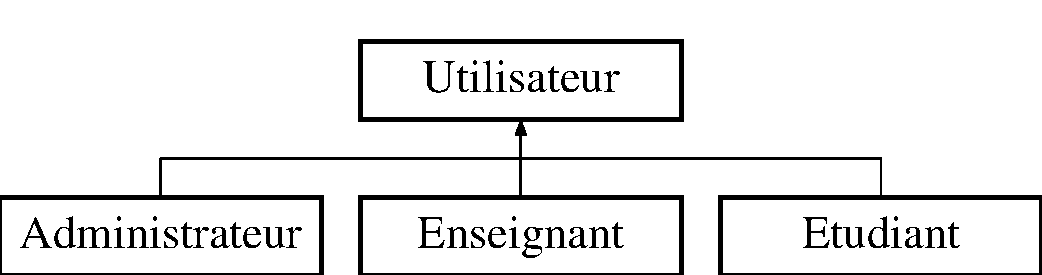
\includegraphics[height=2.000000cm]{classUtilisateur}
\end{center}
\end{figure}
\subsection*{Public Member Functions}
\begin{DoxyCompactItemize}
\item 
\hyperlink{classUtilisateur_a6631539ceecd6140fe525eb91485537b}{$\sim$\-Utilisateur} ()
\begin{DoxyCompactList}\small\item\em Destructeur. \end{DoxyCompactList}\item 
\hypertarget{classUtilisateur_ac71ffe02a37249b5435a630e77703b43}{virtual void \hyperlink{classUtilisateur_ac71ffe02a37249b5435a630e77703b43}{print} ()=0}\label{classUtilisateur_ac71ffe02a37249b5435a630e77703b43}

\begin{DoxyCompactList}\small\item\em Affiche des informations sur l'objet. \end{DoxyCompactList}\end{DoxyCompactItemize}
\subsection*{Protected Member Functions}
\begin{DoxyCompactItemize}
\item 
\hyperlink{classUtilisateur_ae8d5371a46526ec435295ab84cb23555}{Utilisateur} (std\-::string n, std\-::string p, struct tm d)
\begin{DoxyCompactList}\small\item\em Constructeur. \end{DoxyCompactList}\end{DoxyCompactItemize}
\subsection*{Protected Attributes}
\begin{DoxyCompactItemize}
\item 
std\-::string \hyperlink{classUtilisateur_a04d1879dcf1e157f8606cc97b44b0cf6}{nom}
\item 
std\-::string \hyperlink{classUtilisateur_a7cbd4b405cdff4fed665d74ddca1a61f}{prenom}
\item 
struct tm \hyperlink{classUtilisateur_a80d476f8ea3f7ffbbe7e0b8bdd0bb9da}{date\-Naiss}
\end{DoxyCompactItemize}


\subsection{Detailed Description}
Classe utilisateur. 

Cette classe permet de creer un utilisateur (nom/prenom/date naissance) 

\subsection{Constructor \& Destructor Documentation}
\hypertarget{classUtilisateur_ae8d5371a46526ec435295ab84cb23555}{\index{Utilisateur@{Utilisateur}!Utilisateur@{Utilisateur}}
\index{Utilisateur@{Utilisateur}!Utilisateur@{Utilisateur}}
\subsubsection[{Utilisateur}]{\setlength{\rightskip}{0pt plus 5cm}Utilisateur\-::\-Utilisateur (
\begin{DoxyParamCaption}
\item[{std\-::string}]{n, }
\item[{std\-::string}]{p, }
\item[{struct tm}]{d}
\end{DoxyParamCaption}
)\hspace{0.3cm}{\ttfamily [inline]}, {\ttfamily [protected]}}}\label{classUtilisateur_ae8d5371a46526ec435295ab84cb23555}


Constructeur. 

Constructeur de la classe \hyperlink{classUtilisateur}{Utilisateur}


\begin{DoxyParams}{Parameters}
{\em n} & Nom de l'utilisateur \\
\hline
{\em p} & Prénom de l'utilisateur \\
\hline
{\em d} & Date de naissance de l'utilisateur \\
\hline
\end{DoxyParams}
\hypertarget{classUtilisateur_a6631539ceecd6140fe525eb91485537b}{\index{Utilisateur@{Utilisateur}!$\sim$\-Utilisateur@{$\sim$\-Utilisateur}}
\index{$\sim$\-Utilisateur@{$\sim$\-Utilisateur}!Utilisateur@{Utilisateur}}
\subsubsection[{$\sim$\-Utilisateur}]{\setlength{\rightskip}{0pt plus 5cm}Utilisateur\-::$\sim$\-Utilisateur (
\begin{DoxyParamCaption}
{}
\end{DoxyParamCaption}
)\hspace{0.3cm}{\ttfamily [inline]}}}\label{classUtilisateur_a6631539ceecd6140fe525eb91485537b}


Destructeur. 

Detruit un utilisateur (appelé apres le destructeur de la sous classe) 

\subsection{Member Data Documentation}
\hypertarget{classUtilisateur_a80d476f8ea3f7ffbbe7e0b8bdd0bb9da}{\index{Utilisateur@{Utilisateur}!date\-Naiss@{date\-Naiss}}
\index{date\-Naiss@{date\-Naiss}!Utilisateur@{Utilisateur}}
\subsubsection[{date\-Naiss}]{\setlength{\rightskip}{0pt plus 5cm}struct tm Utilisateur\-::date\-Naiss\hspace{0.3cm}{\ttfamily [protected]}}}\label{classUtilisateur_a80d476f8ea3f7ffbbe7e0b8bdd0bb9da}
Date de naissance de l'utilisateur \hypertarget{classUtilisateur_a04d1879dcf1e157f8606cc97b44b0cf6}{\index{Utilisateur@{Utilisateur}!nom@{nom}}
\index{nom@{nom}!Utilisateur@{Utilisateur}}
\subsubsection[{nom}]{\setlength{\rightskip}{0pt plus 5cm}std\-::string Utilisateur\-::nom\hspace{0.3cm}{\ttfamily [protected]}}}\label{classUtilisateur_a04d1879dcf1e157f8606cc97b44b0cf6}
Nom de l'utilisateur \hypertarget{classUtilisateur_a7cbd4b405cdff4fed665d74ddca1a61f}{\index{Utilisateur@{Utilisateur}!prenom@{prenom}}
\index{prenom@{prenom}!Utilisateur@{Utilisateur}}
\subsubsection[{prenom}]{\setlength{\rightskip}{0pt plus 5cm}std\-::string Utilisateur\-::prenom\hspace{0.3cm}{\ttfamily [protected]}}}\label{classUtilisateur_a7cbd4b405cdff4fed665d74ddca1a61f}
Prenom de l'utilisateur 

The documentation for this class was generated from the following file\-:\begin{DoxyCompactItemize}
\item 
\hyperlink{Utilisateur_8hpp}{Utilisateur.\-hpp}\end{DoxyCompactItemize}

\hypertarget{classUtilisateurAbstractFactory}{\section{Utilisateur\-Abstract\-Factory Class Reference}
\label{classUtilisateurAbstractFactory}\index{Utilisateur\-Abstract\-Factory@{Utilisateur\-Abstract\-Factory}}
}
Inheritance diagram for Utilisateur\-Abstract\-Factory\-:\begin{figure}[H]
\begin{center}
\leavevmode
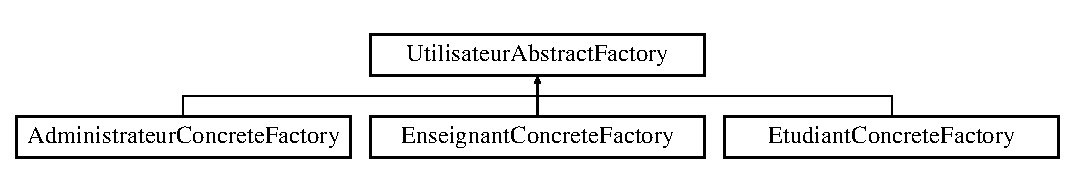
\includegraphics[height=1.895093cm]{classUtilisateurAbstractFactory}
\end{center}
\end{figure}
\subsection*{Public Member Functions}
\begin{DoxyCompactItemize}
\item 
\hypertarget{classUtilisateurAbstractFactory_ac674113eb7df62e4c208bff5d7ec53d3}{virtual \hyperlink{classUtilisateur}{Utilisateur} $\ast$ {\bfseries creer\-Utilisateur} (std\-::string nom, std\-::string prenom)=0}\label{classUtilisateurAbstractFactory_ac674113eb7df62e4c208bff5d7ec53d3}

\end{DoxyCompactItemize}


The documentation for this class was generated from the following file\-:\begin{DoxyCompactItemize}
\item 
\hyperlink{UtilisateurAbstractFactory_8hpp}{Utilisateur\-Abstract\-Factory.\-hpp}\end{DoxyCompactItemize}

\chapter{File Documentation}
\hypertarget{Cours_8hpp}{\section{Cours.\-hpp File Reference}
\label{Cours_8hpp}\index{Cours.\-hpp@{Cours.\-hpp}}
}


Classe cours.  


{\ttfamily \#include $<$string$>$}\\*
{\ttfamily \#include $<$ostream$>$}\\*
\subsection*{Classes}
\begin{DoxyCompactItemize}
\item 
class \hyperlink{classCours}{Cours}
\begin{DoxyCompactList}\small\item\em Classe cours. \end{DoxyCompactList}\end{DoxyCompactItemize}


\subsection{Detailed Description}
Classe cours. \begin{DoxyVersion}{Version}
1d 
\end{DoxyVersion}
\begin{DoxyDate}{Date}
10 décembre 2017 
\end{DoxyDate}

\hypertarget{Enseignant_8hpp}{\section{Enseignant.\-hpp File Reference}
\label{Enseignant_8hpp}\index{Enseignant.\-hpp@{Enseignant.\-hpp}}
}


Classe enseignant.  


{\ttfamily \#include \char`\"{}Utilisateur.\-hpp\char`\"{}}\\*
{\ttfamily \#include \char`\"{}Cours.\-hpp\char`\"{}}\\*
{\ttfamily \#include $<$string$>$}\\*
{\ttfamily \#include $<$ostream$>$}\\*
\subsection*{Classes}
\begin{DoxyCompactItemize}
\item 
class \hyperlink{classEnseignant}{Enseignant}
\begin{DoxyCompactList}\small\item\em Classe enseignant. \end{DoxyCompactList}\end{DoxyCompactItemize}


\subsection{Detailed Description}
Classe enseignant. \begin{DoxyVersion}{Version}
1d 
\end{DoxyVersion}
\begin{DoxyDate}{Date}
10 décembre 2017 
\end{DoxyDate}

\hypertarget{Etudiant_8hpp}{\section{Etudiant.\-hpp File Reference}
\label{Etudiant_8hpp}\index{Etudiant.\-hpp@{Etudiant.\-hpp}}
}


Classe \hyperlink{classEtudiant}{Etudiant}.  


{\ttfamily \#include \char`\"{}Utilisateur.\-hpp\char`\"{}}\\*
{\ttfamily \#include $<$string$>$}\\*
{\ttfamily \#include $<$ostream$>$}\\*
{\ttfamily \#include $<$iostream$>$}\\*
\subsection*{Classes}
\begin{DoxyCompactItemize}
\item 
class \hyperlink{classEtudiant}{Etudiant}
\begin{DoxyCompactList}\small\item\em Classe \hyperlink{classEtudiant}{Etudiant}. \end{DoxyCompactList}\end{DoxyCompactItemize}


\subsection{Detailed Description}
Classe \hyperlink{classEtudiant}{Etudiant}. \begin{DoxyVersion}{Version}
1d 
\end{DoxyVersion}
\begin{DoxyDate}{Date}
10 décembre 2017 
\end{DoxyDate}

\hypertarget{Utilisateur_8hpp}{\section{Utilisateur.\-hpp File Reference}
\label{Utilisateur_8hpp}\index{Utilisateur.\-hpp@{Utilisateur.\-hpp}}
}


Classe abstraite utilisateur.  


{\ttfamily \#include $<$ctime$>$}\\*
{\ttfamily \#include $<$string$>$}\\*
{\ttfamily \#include $<$iostream$>$}\\*
\subsection*{Classes}
\begin{DoxyCompactItemize}
\item 
class \hyperlink{classUtilisateur}{Utilisateur}
\begin{DoxyCompactList}\small\item\em Classe utilisateur. \end{DoxyCompactList}\end{DoxyCompactItemize}


\subsection{Detailed Description}
Classe abstraite utilisateur. \begin{DoxyVersion}{Version}
1d 
\end{DoxyVersion}
\begin{DoxyDate}{Date}
10 décembre 2017 
\end{DoxyDate}

\hypertarget{UtilisateurAbstractFactory_8hpp}{\section{Utilisateur\-Abstract\-Factory.\-hpp File Reference}
\label{UtilisateurAbstractFactory_8hpp}\index{Utilisateur\-Abstract\-Factory.\-hpp@{Utilisateur\-Abstract\-Factory.\-hpp}}
}
{\ttfamily \#include $<$string$>$}\\*
\subsection*{Classes}
\begin{DoxyCompactItemize}
\item 
class \hyperlink{classUtilisateurAbstractFactory}{Utilisateur\-Abstract\-Factory}
\item 
class \hyperlink{classEtudiantConcreteFactory}{Etudiant\-Concrete\-Factory}
\item 
class \hyperlink{classAdministrateurConcreteFactory}{Administrateur\-Concrete\-Factory}
\item 
class \hyperlink{classEnseignantConcreteFactory}{Enseignant\-Concrete\-Factory}
\end{DoxyCompactItemize}


\subsection{Detailed Description}
\begin{DoxyVersion}{Version}

\end{DoxyVersion}
\begin{DoxyDate}{Date}

\end{DoxyDate}

\chapter{Example Documentation}
\hypertarget{console_8cpp-example}{\section{console.\-cpp}
}
Ce programme teste les classes héritant de \hyperlink{classUtilisateur}{Utilisateur}.

À compiler avec la commande 'make -\/f text.\-make'.

\begin{DoxyVersion}{Version}
1a
\end{DoxyVersion}
\begin{DoxyAuthor}{Author}
Luc de Nonancourt
\end{DoxyAuthor}

\begin{DoxyCodeInclude}
\end{DoxyCodeInclude}
 
%--- End generated contents ---

% Index
\newpage
\phantomsection
\addcontentsline{toc}{chapter}{Index}
\printindex

\end{document}
